%(BEGIN_QUESTION)
% Copyright 2010, Tony R. Kuphaldt, released under the Creative Commons Attribution License (v 1.0)
% This means you may do almost anything with this work of mine, so long as you give me proper credit

Beregn spenningen som registreres av analog-til-digital-omformeren inne i temperaturtransmitteren:

$$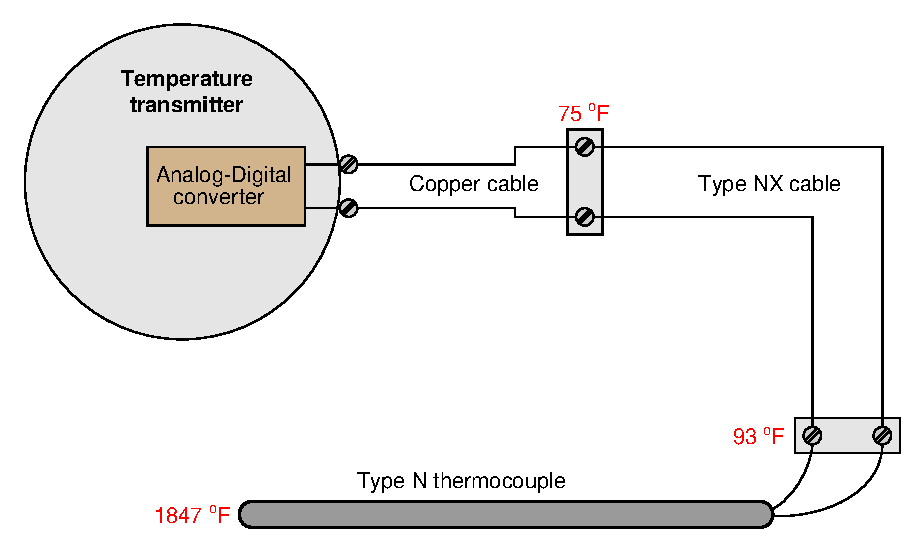
\includegraphics[width=15.5cm]{i00357x01.eps}$$

\underbar{file i00357}
%(END_QUESTION)





%(BEGIN_ANSWER)

Spenning ved ADC: {\bf 35.948} millivolt

\vskip 10pt

Ifølge ITS-90-tabell for type N-termoelementer vil måleskjøten generere 36.577 mV ved 1847 $^{o}$F, mens referanseskjøten (ved NX-kobber-overgangen) vil generere 0.629 mV ved 75 $^{o}$F. Siden vi vet at disse to skjøtespenningene motvirker hverandre, blir spenningen ved transmitterterminalene 35.984 mV.

%(END_ANSWER)





%(BEGIN_NOTES)

%INDEX% Measurement, temperature: thermocouple 

%(END_NOTES)
